\chapter{Research methodology}\label{ch:research-methodology}

The research methodology employed in this thesis adheres to the design science research (DSR) approach, as detailed
in~\cite[p. 17]{rennenkampff_managementitagilitaetentwicklung_2015}.
DSR is a research paradigm where the researcher, acting as a designer, strives to develop artifacts that address
specific problems or questions~\cite[p. 10]{hevner_designscienceresearch_2010}.

In the context of DSR, `design' is defined by Peffers et al. (2007) as the process of crafting an applicable solution
for a given problem~\cite[p.47]{peffers_designscienceresearch_2007}.
As a methodological framework, the design -oriented research approach is particularly well-suited for addressing the
research questions at hand.
The prediction of spring back and bend deduction constitutes a significant issue in practical business applications,
as previously discussed.
Moreover, the development and implementation of machine learning models are inherently design-oriented activities.

% Artifact definition
The term `artifacts' is deliberately broad, encompassing various forms.
In this study, the artifacts refer to machine learning models that are applied to the generated data.
Therefore the term artifact and machine learning model are used interchangeably in this study.

DSR can be executed through diverse means, with a notable example provided by~\cite{peffers_designscienceresearch_2007},
as illustrated in Figure~\ref{fig:dsr_process}.
This approach consists of six steps, which are further divided into the overarching phases of "Build" and "Evaluate".
This thesis adheres to these phases in its research methodology.

\begin{figure}[h]
    \begin{tcolorbox}[arc=0pt,boxrule=0.5pt]
        \centering
        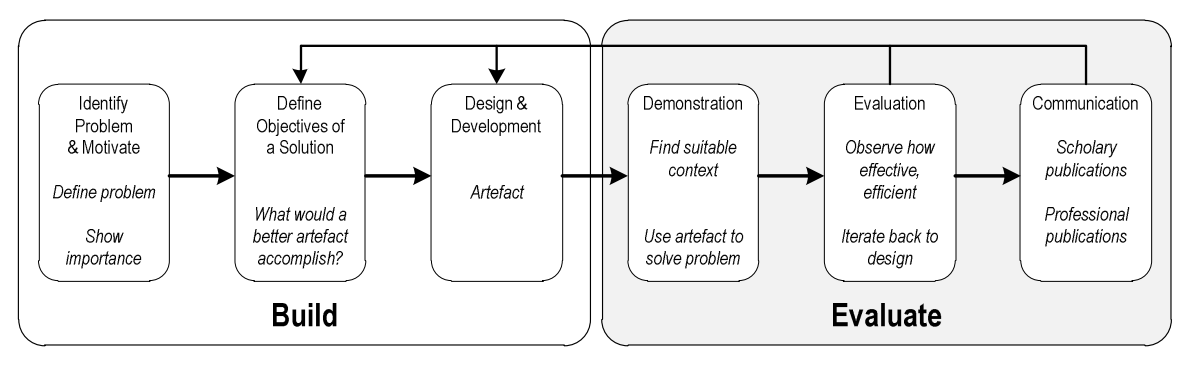
\includegraphics[width=1\linewidth]{chap3/images/dsr_process}
        \caption[DSR Process]{Design Science Research Approach according to Peffers et al.
        Picture:~\cite[p. 72]{sonnenberg_evaluationpatternsdesign_2012}}
        \label{fig:dsr_process}
    \end{tcolorbox}
\end{figure}

\paragraph{``Activity 1 - Problem identification and motivation''~\cite[p. 54]{peffers_designscienceresearch_2007}:}
The specific research problem is identified in this activity and the value of a possible solution is
established~\cite[p. 54--55]{peffers_designscienceresearch_2007}.

The problem as well as the motivation for this study where already described in the chapter~\ref{ch:introduction}
`Introduction' the read an introduction into the topic.
To summarize this study aims to improve the prediction of spring back in the air bending process using real world
data with supervised learning.
The value of the solution will be a reduction of trial and error cycles in the air bending process, which since is done
for example through technology tables.

\paragraph{``Activity 2: Define the objectives for a solution''~\cite[p. 55]{peffers_designscienceresearch_2007}:}
The goal of a solution comes from the definition of the problem, which takes into account what is possible and feasible.
Objectives can be quantitative or qualitative, and they should be based on the problem specification that was
established in the previous step.
Knowledge about previous solutions and their effectiveness is required~\cite[p. 55]{peffers_designscienceresearch_2007}.

The objectives of this study are expressed as six design principles:
correctness,relevance, robustness, stability, resource utilization, and interpretability.
These are explained in detail in the chapter~\ref{sec:objectives-of-a-solution} `Design Principles'.

\paragraph{``Activity 3: Design and development''~\cite[p. 55]{peffers_designscienceresearch_2007}:}
In this phase, the development of the artifact takes place.
An artifact, which may encompass models, methods, or constructs, serves as a critical element in addressing the
research question.
The process begins with outlining the functionality and architecture of the artifacts, followed by their subsequent
creation~\cite[p. 55]{peffers_designscienceresearch_2007}.

In this study the artifacts are machine learning models.
This steps is including the model selection and the training of the models.
The development of the artifacts is described in the chapter~\ref{ch:build} `Build'.

\paragraph{``Activity 4: Evaluation''~\cite[p. 56]{peffers_designscienceresearch_2007}:}
In this activity, the effectiveness of the developed artifact in addressing the defined problems from Activity 1 is
examined and assessed.
The evaluator is expected to have knowledge of relevant metrics and analytical techniques.
The evaluation process may vary based on the nature of the problem at hand which is machine learning in this
study~\cite[p. 56]{peffers_designscienceresearch_2007}.
A comparison between the functionality of the artifact and other existing solutions can be conducted.
Additionally, quantifiable parameters can be employed to objectively measure the artifact's
performance~\cite[p. 56]{peffers_designscienceresearch_2007}.
As already staded in this study the created artifacts are evaluated using six distinct design principles.


\cite{peffers_designscienceresearch_2007} note that researches are not obligated to follow the order of activities
from 1 to 6.
In this study the order fo the activities 4 and 5 are changes.
In the original DSR approach the evaluation is done after the demonstration activity, this was changed because the
evaluation activity is used to select the best performing artifacts.
It would not make sense demonstrate every single machine learning model, because it is expected that not all of them
will perform good enough to employed for the problem.

\paragraph{Activity 5: Demonstration}
The purpose of this activity is to demonstrate the effectiveness of the previously created artifact in solving one or
more problems.
Effective knowledge of the artifact is necessary for this
activity~\cite[p. 55]{peffers_designscienceresearch_2007}.
Unlike the evaluation activity, which assesses the overall performance of the artifact, demonstration focuses on the
performance of the artifact in specific scenarios.
To achieve this, three scenarios, each comprising two examples (single spring back predictions), are utilized to
compare the best -performing models.
The scenarios are selected to cover the entire attribute space of the problem and are described in detail in
Chapter~\ref{ch:evaluation}, \textit{Evaluation}.

\paragraph{Activity 6 - Communication}
The last activity is ued to communicate significance of the problem and the usefulness of the artifacts to a wider
audience~\cite[p. 56]{peffers_designscienceresearch_2007}.
In this study this is done in the chapter~\ref{sec:results-and-discussion} `Results and Discussion'.


\section{Design Principles}\label{sec:design-principles}

% Pado: Do the principles guide the Design&Development step only, or are they used through the
% Build or even Build&Evaluate phases?
% Are there standard principles that should be used, or is there a set to choose from, or does
% one create them individually for each study?

Recent studies suggest that the desired result of design science endeavors should be also be knowledge that takes the
shape of
``Design Principles''~\cite{baskerville2010explanatory, sein2011action, gregor_positioningpresentingdesign_2013}.
They capture knowledge concerning the production of additional examples of objects that belong to the same
category~\cite[p. 39]{sein2011action}.
Other ML models are examples of the same category in the context of this study.
This information is gathered as the researcher progresses from one instance of the artifact to a more general level
~\cite[p. 37]{chandra2016making}.

Design Principles should provide a set of guidelines for the creation of new artifacts.
Also DPs should be abstract enough to be used in later research as well~\cite[p. 37]{sein2011action}.


\section{Evaluation of Machine Learning Models}\label{sec:evaluation-of-machine-learning-models}
Evaluating \ac{ML} models is different from evaluating other software for several reasons.
One of them is that data-driven software components, like \ac{ML} models, have functionality that
is not completely defined by the developer but is instead learned from data.
Therefore, using machine learning presents new challenges compared to traditional software
engineering~\cite[p. 2]{siebert2022construction}.

The field of software engineering has established standards for determining the quality of software systems and their
components.
One such notable standard is the ISO/IEC 9126, which provides a quality model that is widely used in
software engineering.
However, these standards are not applicable for evaluating machine learning models.
Therefore,as noted by Siebert et al. (2022), adaptation is necessary.
They have reinterpreted and expanded upon these existing quality models to make them applicable to the context of
machine learning, as stated in their work~\cite[p. 1]{siebert2022construction}.

In order to define the Design Principles for the \ac{ML} models in this work, the
considerations of~\cite[]{siebert2022construction} are used.
This allows for a systematic process to assess the quality of the developed models.

\cite{siebert2022construction} consider several quality attributes, including
correctness, relevance, robustness, stability, interpretability and resource utilization.
Alongside these attributes, the authors also provide a set of quality measures to evaluate the
models, but these are nor complete and are only used as a starting point for the evaluation of the
models in this work, further evaluation is described in Chapter~\ref{ch:evaluation}.

It is important to note, that the mentioned quality attributes and measures should
not be seen as a complete set of quality attributes and measures for \ac{ML} models.
Other studies, such as~\cite{zhang2020machine} have proposed additional sets of quality attributes.
These additional perspectives will also be considered in the evaluation of the models, but only
as a supplementary means of evaluating model performance.
%In~\cite{zhang2020machine}, the authors describe ``testing properties'' and identify attributes
%such as correctness, relevance, robustness, and interpretability, which are similar to those
%mentioned in~\cite{siebert2022construction}.
%However, this work does not consider attributes such as Security, Fairness, and Privacy~\cite[p.
%3]{zhang2020machine}, as they may be difficult to measure and in the context of sheet metal
%bending they are not relevant for this work.


\section{Goal Question Metric Approach}\label{subsec:goal-question-metric-approach}
To make the defined quality attributes measurable, the “Goal-Question-Metric”-approach \ac{GQM}
was chosen in this work.
It is one of the most common approaches in DSR and is divided into three levels~\cite[p. 3]{basili_goalquestionmetric_}.

\paragraph{1. Conceptual level (goal):}
``A goal is defined for an object, for a variety of reasons,
with respect to various models of quality, from various points of view, relative to a
particular environment.''~\cite[p. 3]{basili_goalquestionmetric_}

Specific goals are established for a software product (in this case a \ac{ML} model).
These goals consider various quality aspects, perspectives, and contexts.
Clearly defined goals help to guide the direction of the development~\cite[p. 3]{basili_goalquestionmetric_}.

\paragraph{2. Operational level (question):}
To achieve the set goals, one ore multiple questions are fomrulated to asses and characterize the objectives.
These questions address the quality attributes and help understanding the object of measurement from the selected
viewpoint.
The questions guide the measurement process by identifying the relevant aspects that need to be
analyzed~\cite[p. 3]{basili_goalquestionmetric_}.

\paragraph{3. Quantitative level (metric):}
For each question, a set of metrics is defined to provide quantitative data and answers.
These metrics are used to evalute the object of measurement, offering precise and objective insights into the
quality aspects being assessed~\cite[p. 3]{basili_goalquestionmetric_}.

In this study only one question is formulated for each goal.
The goals, questions and metrics are presented in the next chapter.
